%% main_rtai_artigo.tex, based on abtex2-modelo-Artigo.tex, v-1.9.6 laurocesar 
%% Adaptado por Prof. Dr. Renato Kazuo Miyamoto 
%% Departamento de Elétrica e Automação
%% Centro Universitário UNISENAI Londrina

%% Copyright 2012-2016 by abnTeX2 group at http://www.abntex.net.br/ 

% ------------------------------------------------------------------------
% ------------------------------------------------------------------------
% abnTeX2: Modelo de Artigo Acadêmico em conformidade com
% ABNT NBR 6022:2003: Informação e documentação - Artigo em publicação 

% ------------------------------------------------------------------------
% ------------------------------------------------------------------------

\documentclass[
% -- opções da classe memoir --
article,			% indica que é um artigo acadêmico
11pt,				% tamanho da fonte
twoside,			% para impressão apenas no recto. Oposto a twoside
a4paper,			% tamanho do papel
% -- opções da classe abntex2 --
%chapter=TITLE,		% títulos de capítulos convertidos em letras maiúsculas
section=TITLE,		% títulos de seções convertidos em letras maiúsculas
%subsection=TITLE,	% títulos de subseções convertidos em letras maiúsculas
%subsubsection=TITLE % títulos de subsubseções convertidos em letras maiúsculas
% -- opções do pacote babel --
onecolumn,          % texto em duas colunas
english,			% idioma adicional para hifenização
brazil,				% o último idioma é o principal do documento
sumario=tradicional
]{abntex2}

\usepackage{sty/packs}

% ----
% Se necessário, inclua outros pacotes aqui
\usepackage[utf8]{inputenc}
\usepackage{hyperref}
\usepackage{graphicx}
\usepackage[alf]{abntex2cite}	% Citações padrão ABNT
\usepackage{footmisc} % para melhorar formatação das notas de rodapé
% ---
\begin{document} 
% ---
% Informações de dados para CAPA e FOLHA DE ROSTO
% ---
% Título
\begin{center}
   
    {\bfseries TÍTULO: subtítulo em língua vernácula} \\
   
    \vspace{0.5cm}

\end{center}



% Autores alinhados à direita
\begin{flushright}
    \fontsize{7}{9}\selectfont
    Angelo Aparecido Salvador Avelino\footnotemark[1] \quad   \\
    Gabriel Gonçalves Costa\footnotemark[2] \quad \\
    Huan Radov Luchetti\footnotemark[3] \quad  \\
    Lucas Vinicius de Bortoli Santos\footnotemark[4] \quad  \\
    Pedro Antônio Frasson\footnotemark[5] \quad  \\
    Vinicius de Morais Boim dos Santos\footnotemark[6] \quad  \\
    Cinthya Oestreich Silva (Orientador)\footnotemark[7] \\
\end{flushright}

\vspace{1cm}

% Definindo as notas de rodapé para cada autor
\footnotetext[1]{UniSENAI PR, gab.gabriel.1003@outlook.com}
\footnotetext[2]{UniSENAI PR, email, etc.)}
\footnotetext[3]{UniSENAI PR, email, etc.)}
\footnotetext[4]{UniSENAI PR, email, etc.)}
\footnotetext[5]{UniSENAI PR, email, etc.)}
\footnotetext[6]{UniSENAI PR, email, etc.)}
\footnotetext[7]{UniSENAI PR, email, etc.)}

\vspace{1cm}

%\local{Brasil}
%\data{ Departamento de Engenharia Elétrica e Automação Industrial \\ Centro Universitário UniSenai PR \\ Londrina/PR - Brasil - Janeiro 2025, v-1.0}
% ---

% ----
% Início do documento
% ----

    
    % Seleciona o idioma do documento (conforme pacotes do babel)
    %\selectlanguage{english}
    \selectlanguage{brazil}
    
    % Retira espaço extra obsoleto entre as frases.
    \frenchspacing 
    
    % ----------------------------------------------------------
    % ELEMENTOS PRÉ-TEXTUAIS
    % ----------------------------------------------------------
    
    %\twocolumn[    		% INICIO DE ARTIGO EM DUAS COLUNAS
    
    % página de titulo
   % \maketitle
    % resumo em português
    \begin{resumo}
        Conforme a ABNT NBR 6022:2003, o resumo é elemento obrigatório, constituído de uma sequência de frases concisas e objetivas e não de uma simples enumeração de tópicos, não ultrapassando 250 palavras, seguido, logo abaixo, das palavras representativas do conteúdo do trabalho, isto é, palavras-chave e/ou descritores, conforme a NBR 6028. (\ldots) As palavras-chave devem figurar logo abaixo do resumo, antecedidas da expressão Palavras-chave:, separadas entre si por ponto e finalizadas também por ponto.
        \noindent
        
        \textbf{Palavras-chave}: IoT. LoRa. Edge Computing. Smart Cities.
    \end{resumo}
        
    % resumo em português
    \renewcommand{\resumoname}{Abstract}
    \begin{resumo}
        \begin{otherlanguage*}{english}
            According to ABNT NBR 6022:2003, an abstract in foreign language is a back
            matter mandatory element.
            
            \noindent
            \textbf{Keywords}: information. Logic. Technology. Architecture of Information.
        \end{otherlanguage*}  
    \end{resumo}
    
    
    \vspace{\onelineskip}%
    
  %  ]  				% FIM DE ARTIGO EM DUAS COLUNAS
    % ---
    
    
    % ----------------------------------------------------------
    % ELEMENTOS TEXTUAIS
    % ----------------------------------------------------------
    \textual
    
    % ----------------------------------------------------------
    % Introdução
    % ----------------------------------------------------------
    \section{Introdução}
    \addcontentsline{toc}{section}{Introdução}
    
    Este documento e seu código-fonte são exemplos de referência de uso da classe \textsf{abntex2} e do pacote \textsf{abntex2cite}. O documento exemplifica a elaboração de publicação periódica científica impressa produzida conforme a ABNT NBR 6022:2003 \emph{Informação e documentação - Artigo em publicação periódica científica impressa - Apresentação}.
    
    A expressão ``Modelo canônico'' é utilizada para indicar que \abnTeX\ não é modelo específico de nenhuma universidade ou instituição, mas que implementa tão somente os requisitos das normas da ABNT. Uma lista completa das normas observadas pelo \abnTeX\ é apresentada em \citeonline{abntex2classe}.
    
    Sinta-se convidado a participar do projeto \abnTeX! Acesse o site do projeto em \url{http://www.abntex.net.br/}. Também fique livre para conhecer, estudar, alterar e redistribuir o trabalho do \abnTeX, desde que os arquivos modificados tenham seus nomes alterados e que os créditos sejam dados aos autores originais, nos termos da ``The \LaTeX\ Project Public License''\footnote{\url{http://www.latex-project.org/lppl.txt}}.
    
    Encorajamos que sejam realizadas customizações específicas deste documento. Porém, recomendamos que ao invés de se alterar diretamente os arquivos do \abnTeX, distribua-se arquivos com as respectivas customizações. Isso permite que futuras versões do \abnTeX~não se tornem automaticamente incompatíveis com as customizações promovidas. Consulte \citeonline{abntex2-wiki-como-customizar} par mais informações.
    
    Este exemplo deve ser utilizado como complemento do manual da classe \textsf{abntex2} \cite{abntex2classe}, dos manuais do pacote \textsf{abntex2cite} \cite{abntex2cite,abntex2cite-alf} e do manual da classe \textsf{memoir} \cite{memoir}. Consulte o \citeonline{abntex2modelo} para obter exemplos e informações adicionais de uso de \abnTeX\ e de \LaTeX.

A introdução deve apresentar uma visão geral do artigo, delimitando o tema e o problema a ser abordado, bem como o (s) objetivo (s) e a justificativa. O intuito é chamar a atenção do leitor para o assunto que será apresentado no artigo, sem aprofundar conceitos ou antecipar resultados. 

O corpo do texto, salvo exceções que serão mencionadas no decorrer do documento, devem ser grafados em fonte tamanho 12 pts, tipo Arial, espaçamento entre linhas de 1,5 com 0 pts. antes e 0 pts. depois. O alinhamento do texto deve ser “justificado”, e as margens devem figurar -  3 cm para margem superior e esquerda; e 2 cm para margem inferior e direita. O parágrafo (recuo esquerdo) deve ser de 1,25 cm. No artigo o texto deve ser apresentado sequencialmente, não ocorrendo quebra de página quando se inicia um novo capítulo e ou seção bem como seguir padrão adotado de espaçamento conforme apresenta-se a seguir: a) Entre o título e o início da seção, deve-se atribuir um espaço; b) Ao final de cada seção deve-se atribuir um espaço para iniciar um novo capítulo e ou seção ou subseção. 

    % ----------------------------------------------------------
    % Seção de explicações
    % ----------------------------------------------------------
\section{Fundamentação teórica}

Parte que embasa cientificamente o trabalho. Deve-se expor o assunto tratado de forma pormenorizada e ordenada, divide-se em seções e subseções de acordo com o tipo de trabalho. A seção Fundamentação teórica, assim como as demais seções e subseções devem ser separadas do texto que a antecede e que a precede por 1 (um) espaço de entrelinhas de 1,5 cm.

Todas as fontes de informação usadas devem ser citadas, conforme as orientações da ABNT NBR 10520 (2023). 

Essa seção não deve contemplar opiniões, experiências pessoais e/ou dados ou resultados da pesquisa de campo do referido estudo. Ela deve ser usada exclusivamente para apoiar bibliograficamente a temática do estudo/artigo.

Priorize as citações indiretas em relação às citações diretas e quando não tiver acesso ao texto original use a regra da ABNT NBR 10520 (2023) apud - citação de citação.

Para palavras e/ou termos estrangeiras no texto, utilizar itálico. 
De forma a facilitar a apresentação das citações na sequencia seguem exemplos dos dois modelos mais usados – citação indireta e citação direta, conforme ABNT NBR 10520 (2023).
Citação indireta  (conceitual ou paráfrase) texto baseado na obra do autor consultado. Não usar aspas e não é obrigatório apresentar páginação.

Exemplo:  Segundo Foster (2011) depois de aprender e armazenar novas informações podemos selecionar, interpretar, e integrar uma coisa à outra – para fazer um melhor uso do que aprendemos e lembramos.

Citação direta (literal ou textual) é a transcrição de palavras ou trechos de outro autor e podem ser apresentadas de duas maneiras:
Exemplo - Citação direta (breve) - citação com menos de três linhas, autor inserido no texto usando aspas (“”)

Exemplo 1 - a) Segundo Santos (2018, p. 240) “[...] trecho do texto do autor citado tal e qual a obra original.” b) Quando a autoria for apresentada no final da citação, observar o seguinte exemplo: “[...] trecho do autor citado tal e qual obra original.” (Santos, 2018, p. 240)

Exemplo 2 -  citação direta, com mais de três linhas ,deve ser destacada com recuo padronizado em relação à margem esquerda, com letra menor que a utilizada no texto, em espaçamento simples e sem aspas. Recomenda-se o recuo de 4cm. ABNT NBR 10520 (2023).
    
    \begin{citacao}
        \lipsum[2]
    \end{citacao}
    
    \lipsum[3]

    
    \subsection{Título secundário}
    
  (Subdivisão do texto a partir de uma seção primária) Exemplo: 2.1 Assunto de relação dentro do assunto primário / 2.2 Assunto de relação dentro do assunto secundário). Consulte ABNT NBR 6024 (2012).

  \subsubsection{Título terciário}
(Subdivisão do texto a partir de uma seção secundária) 
Exemplo: 2.1.1 Assunto de relação dentro do assunto secundário/ 2.1.2 Assunto de relação dentro do assunto secundário). Consulte ABNT NBR 6024 (2012)

O autor tem liberdade para nomear as subdivisões como achar conveniente para o trabalho, devendo apenas evitar tópicos considerados curtos (menos de meia página). 
É importante lembrar que os trabalhos acadêmicos requerem um encadeamento lógico e muito embora ilustrações contribuam significativamente para a compreensão do trabalho e melhor priorizar a exposição das ideias.

**Importante: O texto deve ser precedidos ou antecedidos de comentários, conforme exemplo a seguir: “O Quadro 1 demonstra [...]” – (não usar: “A seguir” / “Abaixo”).

Segundo a ABNT NBR 14724 (2011), qualquer que seja o tipo (desenho esquema, fluxograma, fotografia, gráfico, mapa, organograma, planta, quadro, retrato, figura, imagem, entre outros) sua identificação deverá aparecer na parte superior, precedida da palavra designativa, seguida de seu número de ordem de ocorrência no texto, em algarismos arábicos, travessão e do respectivo título de forma centralizada. Após a ilustração, na parte inferior, indicar a fonte consultada (elemento obrigatório, mesmo que seja produção do próprio autor), legenda, notas e outras informações necessárias à sua compreensão (se houver) de forma alinhada a esquerda da ilustração apresentada. A ilustração devem ser padronizadas, devem ser citadas no texto seguindo o sistema autor-data conforme NBR 10520 (2023), bem como estar inseridas o mais próximo possível do trecho a que se refere.

Exemplo de lista de itens numerada:
\begin{enumerate}
\item Item numerado 1.
\item Item numerado 2.
\item Item numerado 3.
\item Item numerado 4.
\item Item numerado 5.
\end{enumerate}

A equação (\ref{eq:fx}) é um exemplo de equação inserida usando o ambiente LaTeX e numerada automaticamente.

\begin{equation}
\label{eq:fx}
f(x) = \frac{1}{\alpha} \int_0^L \left(\frac{x^2}{2} -\frac{x^3}{3}\right) \mathrm{d} x
\end{equation}


A Figura \ref{fig1} é um exemplo de figura inserida usando o ambiente LaTeX e numerada automaticamente.

\begin{figure}[!htb]
\centering%
\caption{Título da figura.}%
\label{fig1}
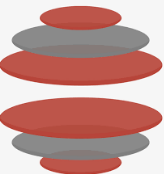
\includegraphics[width = 0.5\columnwidth]{figuras/Imagem1.png}
\\Fonte: Autoria própria.
\end{figure}

A Tabela 1 \ref{tab:Ldimens} é um exemplo de tabela inserida usando o ambiente LaTeX e numerada automaticamente.

\begin{table}[!htb]
\centering%
\small%
\caption{Exemplo de legenda de tabela.}%
\label{tab:Ldimens}
\begin{tabular*}{\columnwidth}{@{\extracolsep{\fill}}cccc}
\toprule
$L$   & $L^2$     & $L^3$     & $L^4$     \\
{[m]} & {[m$^2$]} & {[m$^3$]} & {[m$^4$]} \\
\midrule
1     & 1         & 1         & 1         \\
2     & 4         & 8         & 16        \\
3     & 9         & 27        & 81        \\
4     & 16        & 64        & 256       \\
5     & 25        & 125       & 625       \\
\bottomrule
\addlinespace
\end{tabular*}
\\Fonte: Autoria própria.
\end{table}

    
\section{Metodologia}
    
Aqui deve-se descrever a metodologia utilizada no trabalho. Sugere-se a seguinte estrutura: classificação do tipo da pesquisa (quanto aos fins e quanto aos meios); descrição de onde foi feita a pesquisa (unidade de análise ou universo e amostra); informações sobre a coleta dos dados (detalhamento dos instrumentos de coleta e procedimentos utilizados) e explicações sobre como os analisou (pesquisa qualitativa e/ou quantitativa).

É importante detalhar especificamente o protocolo utilizado na coleta de dados: explique se houve realização de entrevistas ou aplicação de questionário. Cite a fonte do questionário/formulário, caso não tenha sido elaborado exclusivamente para essa pesquisa; explique quem e quantos foram os entrevistados ou pesquisados, como os escolheu, como e quando ocorreu a pesquisa. 

Explique se houve coleta de dados documental (acesso a documentos ou sistema de alguma empresa ou instituição), como e porque ocorreu tal coleta; explique se houve coleta de dados por observação (filmagens, por exemplo), como e porque ocorreu tal coleta; explique se houve realização de testes, experimentos ou construção de equipamentos em bancadas, laboratórios ou oficinas (como e onde ocorreu). Essa seção deve ter no máximo duas páginas.

\section{Apresentação de discussão dos resultados}
Nessa seção devem constar os resultados encontrados na pesquisa, visando cumprir os objetivos propostos, através da metodologia especificada na seção anterior. É facultado ao autor dividir essa seção em subseções conforme ABNT NBR 6024 (2012). 
(Caso sua pesquisa seja uma Pesquisa Bibliográfica use como título desta seção apenas Discussão)



    % ---
    % Finaliza a parte no bookmark do PDF, para que se inicie o bookmark na raiz
    % ---
    \bookmarksetup{startatroot}% 
    % ---
    
    % ---
    % Conclusão
    % ---
 \section{Considerações finais}
 \addcontentsline{toc}{section}{Considerações finais}
 Parte final do artigo, na qual o autor evidencia que os objetivos foram cumpridos, destaca os principais resultados obtidos e deixa sugestões para estudos futuros acerca do tema estudado.
 
Na conclusão não se utiliza citações, ilustrações e não se apresenta resultados ou conceitos novos (que não haviam sido apresentados anteriormente no texto).

    
        
    % ----------------------------------------------------------
    % ELEMENTOS PÓS-TEXTUAIS
    % ----------------------------------------------------------
    \postextual                 % Os elementos pós-textuais estão desabilitados nesse modelo
    
    % ----------------------------------------------------------
    % Referências bibliográficas
    % ----------------------------------------------------------
    \bibliography{rtai}
    
    % ----------------------------------------------------------
    % Glossário
    % ----------------------------------------------------------
    %\glossary
    
    % ----------------------------------------------------------
    % Apêndices
    % ----------------------------------------------------------
    \vspace{1cm}
    \begin{apendicesenv}
        
        % ----------------------------------------------------------
        \chapter{Nullam elementum urna vel imperdiet sodales elit ipsum pharetra ligula
            ac pretium ante justo a nulla curabitur tristique arcu eu metus}
        % ----------------------------------------------------------
        \lipsum[55-57]
        
    \end{apendicesenv}
    % ---
    
    % ----------------------------------------------------------
    % Anexos
    % ----------------------------------------------------------
    \cftinserthook{toc}{AAA}
    \vspace{1cm}
    \begin{anexosenv}
        
        % ---
        \chapter{Cras non urna sed feugiat cum sociis natoque penatibus et magnis dis
            parturient montes nascetur ridiculus mus}
        % ---
        
        \lipsum[31]
        
    \end{anexosenv}
\end{document}
